% !TEX root =  ../main.tex 

\section{Simulation study}
\label{sec: simulation_study}
The application of personalized schedules for patients in PRIAS demonstrated that personalized schedules adapt according to the PSA and repeat biopsy history of each patient. However, since the patients in PRIAS have already had their biopsies as per the PRIAS schedule, we were not able to evaluate the efficacy of personalized schedules against the PRIAS schedule. To this end, we have performed a simulation study to compare 3 broad categories of schedules: Personalized schedules, PRIAS schedule and the schedule of annual biopsy. In the simulation study we simulate the progression of patients enrolled in an AS program. The PSA measurements are measured periodically as per a fixed schedule, however the biopsies are conducted as per the scheduling algorithms until GR is detected. We next present the details of the simulation study and the biopsy schedule evaluation criteria.

\subsection{Simulation setup}
\label{subsec : simulation_setup}
\subsubsection{Patient population}
For the simulation study we first select a population $\mathcal{P}$ of patients enrolled in AS. We assume that the PSA and hazard of GR for the patients from this population follows a joint model of the form postulated in Section \ref{subsec : jm_fit_prias}. The population parameters $\boldsymbol{\theta}^{\mathcal{P}}$ are selected to be equal to the posterior mean of parameters $E[\boldsymbol{\theta} \mid \mathcal{D}^{PRIAS}]$ estimated from the joint model fitted to PRIAS data set (Section \ref{subsec : param_estimates_jm_fit_prias}). To demonstrate the efficacy of personalized schedules for patients with early as well late failure times, we ensured that the patients in population $\mathcal{P}$ were from 3 equal sized sub-groups. The baseline hazard for each of the sub-group was assumed to be the hazard function for a Weibull distribution. The shape and scale parameters $(k, \lambda$) for the aforementioned Weibull distribution are $(1.5, 4)$, $(3, 5)$ and $(4.5, 6)$.

\subsubsection{Simulated data sets}
From the population $\mathcal{P}$ we randomly sample a total of 200 data sets with 1000 patients each. For each of the patients, the longitudinal profiles for PSA scores are generated as per the visiting schedule of PRIAS study. i.e. Every 3 months for first 2 years and every 6 months thereafter. The true GR reclassification times are also generated. We then divide each of the 200 simulated data sets into training (750 patients) and test (250 patients) parts. Further we generate random and non-informative censoring times for the patients in 200 training data sets $\mathcal{D}^1, \ldots \mathcal{D}^{200}$. The observed data in the $k^{th}$ training data set is $\mathcal{D}^k = \{T_{ki}, \delta_{ki}, \boldsymbol{y}_{ki}; i = 1,\ldots 750\}$, where $\boldsymbol{y}_{ki}$ denotes the PSA measurements for the $i^{th}$ patient in the $k^{th}$ training data set. $T_{ki} = \min(T^*_{ki}, C_{ki})$ denotes the observed GR time whereas the true GR time and censoring times are denoted by $T^*_{ki}$ and $C_{ki}$ respectively. $\delta_{ki} = I(T^*_{ki} < C_{ki})$ is the event indicator, where $I(\cdot)$ is an indicator function that takes the value 1 when $T^*_{ki} < C_{ki}$ and 0 otherwise. For the patients in the test data sets no censoring times are generated.

\subsubsection{Personalized schedules for test patients}
\label{subsubsec : sim_study_pers_sched_details}
We create personalized biopsy schedules only for the patients in the test data set. To this end we first fit a joint model to the training data set to obtain posterior estimates of parameters $p(\boldsymbol{\theta} \mid \mathcal{D}^k)$, which are required for the posterior predictive distribution $g(T^*_{kj})$ of the $j^{th}$ patient from the $k^{th}$ test data set. To model the baseline hazard we use a P-splines approach (Section \ref{subsec : jm_specification}). While the posterior predictive distribution is sufficient for scheduling biopsies based on expected time of GR, the choice of time window $\Delta t$ (Section \ref{subsubsec : dynamic_risk_definitions}) has to be made for scheduling biopsies on the basis of dynamic risk of GR. In PRIAS and in most AS programs biopsies are done at a gap of 1 to 3 years. A gap of 1 year between biopsies detects GR the earliest, and in worst case the detection of GR can be delayed by 1 year. Being a clinically relevant period of time to differentiate between patients who obtain GR and those who don't, we choose a $\Delta t$ of 1 year. In schedules based on dynamic risk of GR, for a test patient $j$, we choose a value of $\kappa$ which maximizes a binary classification measure (Section \ref{subsubsec : kappa_estimation}) at the last known repeat biopsy time $t$ of the patient. To this end the binary classification measures are first computed over a fine grid of values in the interval $[0,1]$ using the training data set and then the most optimal $\kappa$ is chosen.\\

To create personalized schedules we employ the algorithm described in Section \ref{subsec : pers_sched_algorithm}. The algorithm is run for 7 different settings, one each corresponding to the following: PRIAS schedule, annual biopsy schedule, expected time of GR, median time of GR, dynamic risk of GR with $\kappa$ chosen such that a) Youden index is maximized, b) F1 score is maximized. In addition to these a mixed approach is also employed where at any point in time......

\subsection{Evaluating efficacy of scheduling methods}
For a particular biopsy scheduling method $S$, the first criteria in the evaluation of efficacy of the method is the number of repeat biopsies $N^{bS}$ it takes before GR is detected for a patient from the population. The less the $N^{bS}$ the better it is for patients. Our interest lies in the marginal distribution of $N^{bS}$ for the population $\mathcal{P}$. Since In its simplest form, the mean $E[N^{bS}]$ and variance $Var[N^{bS}]$ of the aforementioned distribution indicate the performane of the scheduling algorithm. More specifically, a low mean as well as low variance is desired. Other quantiles of the distribution may also be used evaluation criteria. For e.g. a method which takes less than 2 (say) biopsies in 95\% cases may be desriable.\\

The second criteria in evaluation of efficacy of a schedule is the offset. Given a schedule $S$, the offset for a particular patient $j$ is defined as $O^S_j = T^S_{j{N^{bS}_j}} - T^*_j$, where $N^{bS}_j$ is the number of biopsies required for patient $j$ before GR is detected and $T^S_{j{N^{bS}_j}} > T^*_j$ is the time at which GR is detected by the scheduling mechanism $S$. Once again the interest lies in both the mean $E[O^S]$ and variance $Var[O^S]$ of the marginal distribution of offset.

\subsubsection{Finding the most optimal schedule}
Given the multiple evaluation criteria the next step is to find the most optimal schedule. Using principles from compound optimal designs \citep{lauter1976optimal} we propose to choose a schedule $S$ which minimizes the following loss function:

\begin{equation}
\label{eq : loss_func_sim_study_generic}
L(S) = \sum_{g=1}^G \lambda_g \mathcal{G}_g(N^{bS})^{d_g=1}\mathcal{G}_g(O^S)^{d_g=0}
\end{equation}
where $\mathcal{G}_g(\cdot)$ is either a function of number of biopsies or of the offset, and $d_g$ is the corresponding indicator for this choice. Some examples of $\mathcal{G}_g(\cdot)$ are mean, median, variance and quantile function. Constants $\lambda_1, \ldots \lambda_G$, where $\lambda_g \epsilon [0,1]$ and $\sum_{g=1}^G \lambda_g = 1$, are weights to differentially weigh-in the contribution of each of the $G$ evaluation criteria manifested via the functions $\mathcal{G}_g(\cdot)$. An example loss function is:

\begin{equation}
\label{eq : loss_func_sim_study}
L(S) = \lambda_1 E[N^{bS}] + \lambda_2 E[O^S] 
\end{equation}
The choice of $\lambda_1$ and $\lambda_2$ is not easy. This because biopsies have serious medical side effects and the cost of an extra biopsy cannot be quantified easily. To obviate this issue we utilize the equivalence between compound and constrained optimal designs \citep{cook1994equivalence}. More specifically, it can be shown that for any $\lambda_1$ and $\lambda_2$ there exists a constant $C>0$ for which minimization of loss function in Equation \ref{eq : loss_func_sim_study} is equivalent to minimization of the same, subject to the constraint that $E[O^S] < C$. i.e. The optimal schedule is the one with the least number of biopsies and an offset less than $C$. The choice of $C$ now can be based on the protocol of AS program. For e.g. in PRIAS the maximum gap between 2 repeat biopsies is 3 years. i.e. If GR is detected within 3 years of its occurance, it is acceptable by the AS program. For a more general scenario of the form in Equation \ref{eq : loss_func_sim_study_generic}, the solution can be found by minimizing $\mathcal{G}_G(\cdot)$ under the constraint $\mathcal{G}_g < C_g; g=1, \ldots G-1$.\\

In this work, we estimate $E[N^{bS}]$, $Var[N^{bS}]$, $E[O^S]$ and $Var[O^S]$ using pooled estimates of each from the 200 repetitions of the simulation study. The estimates are calculated separately for each of the 7 methods mentioned in Section \ref{subsubsec : sim_study_pers_sched_details}. The pooled estimates for a scheduling method $S$ are calculated as following:

\begin{align*}
\widehat{E[O^S]} &= \frac{\sum_{k=1}^{200} n_k \widehat{E[O^S_k]}}{\sum_{k=1}^{200} n_k}, \\
\widehat{Var[O^S]} &= \frac{\sum_{k=1}^{200} (n_k - 1) \widehat{Var[O^S_k]}}{\sum_{k=1}^{200} (n_k-1)}, 
\end{align*}
where $n_k$ are the number of test patients in the $k^{th}$ simulation, $\widehat{E[O^S_k]} = \frac{\sum_{j=1}^{n_k}O^S_{kj}}{n_k}$ and $\widehat{Var[O^S_k]} = \frac{\sum_{j=1}^{n_k}(O^S_{kj} - \widehat{E[O^S_k]})^2}{n_k-1}$ are the estimated mean offset and estimated variance of the offset for the $k^{th}$ simulation, respectively. The estimates for number of biopsies $N^{bS}$ are calculated similarly.

\subsection{Results}
The pooled estimates of the mean and variance of number of biopsies as well as offset from the simulation study are summarized in Table \ref{table : sim_study_pooled_estimates}. We can see that schedules based on Expected time of GR and Median time of GR schedule on an average 2 biopsies before GR is detected and the variance in number of biopsies is very low. On the other hand PRIAS and annual biopsy schedule 4 or more biopsies for the same and the variance in number of biopsies is high. As expected the higher number of biopsies lead to a smaller offset as well. For e.g. annual biopsy schedule has an average offset of 6 months and has a low variance as well. The average offset for Expected and Median time of GR is approximately 13 to 14 months, which is acceptable time period in PRIAS. The variance of the offset is high though. In a nutshell methods which conduct high number of biopsies have less variance in offset. In this regard the mixed approach (\Section \ref{subsec : mixed_approach}) lies between the two extremes since it conducts 3 biopsies on average and has low variance for offset as well for number of biopsies. Furthermore, the average offset is also less than an year for this approach. Lastly, in Figure \ref{fig : nbBoxPlot} and Fig \ref{fig : offsetBoxPlot} we show a boxplot of number of biopsies and offset for all of the 250 * 200 patients in the simulation study. WHY IS THIS BOXPLOT HERE...DISCUSS IT.

% Please add the following required packages to your document preamble:
% \usepackage{booktabs}
\begin{table}[!htb]
\centering
\captionsetup{justification=centering}
\caption{Pooled estimates of mean and variance of number of biopsies and offset for the simulation study.}
\label{table : sim_study_pooled_estimates}
\begin{tabular}{@{}lrrrrr@{}}
\toprule
               & Total Patients & $E[N^{bS}]$ & $Var[N^{bS}]$ & $E[O^S]$ & $Var[O^S]$ \\ \midrule
Annual         & 387            & 4.307                           & 10.426                            & 5.973                      & 11.886                       \\
F1score        & 395            & 4.658                           & 4.303                             & 6.731                      & 16.101                       \\
Expected Time of GR           & 379            & 1.997                           & 1.405                             & 13.764                     & 115.228                      \\
Median Time of GR         & 395            & 2.056                           & 1.670                             & 14.271                     & 136.769                      \\
Mixed.Approach & 387            & 3.220                           & 5.074                             & 10.496                     & 65.175                       \\
PRIAS          & 387            & 4.054                           & 8.812                             & 7.663                      & 50.295                       \\
Youden         & 379            & 4.625                           & 3.594                             & 8.900                      & 231.035                      \\ \bottomrule
\end{tabular}
\end{table}

\begin{figure}[!htb]
	\centering
    \captionsetup{justification=centering}
	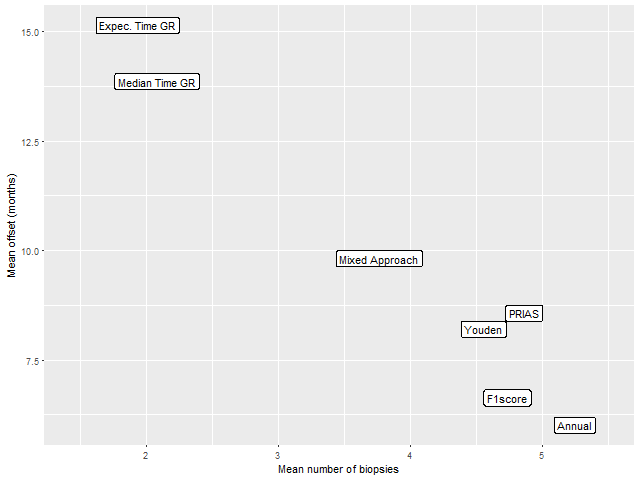
\includegraphics[width=0.8\textwidth]{images/sim_study/meanNbVsOffset.png}
	\caption{Estimated mean number of biopsies and mean offset (months) for the 7 scheduling methods.}
	\label{fig : meanNbVsOffset}
\end{figure}

\begin{figure}[!htb]
    \centering
    \captionsetup{justification=centering}
     \begin{subfigure}[b]{0.45\textwidth}
        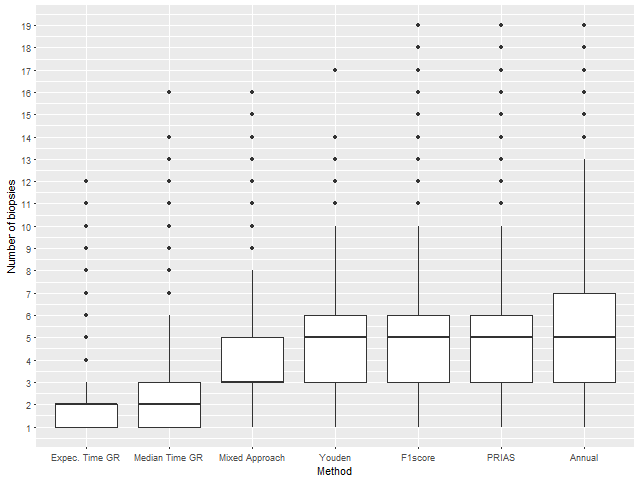
\includegraphics[width=\textwidth]{images/sim_study/nbBoxPlot.png}
        \caption{Boxplot for number of biopsies.}
        \label{fig : nbBoxPlot}
    \end{subfigure}
    \begin{subfigure}[b]{0.45\textwidth}
        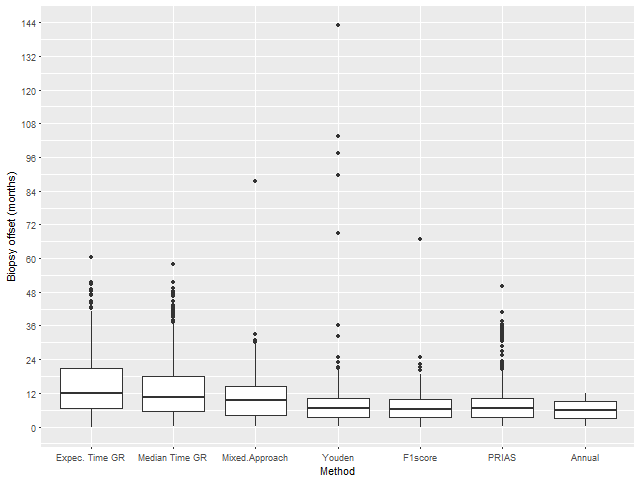
\includegraphics[width=\textwidth]{images/sim_study/offsetBoxPlot.png}
        \caption{Boxplot for offset (months)}
        \label{fig : offsetBoxPlot}
    \end{subfigure}      
    \caption{Boxplot for number of biopsies and offset (months), for all the patients in the 200 simulated data sets.}
\end{figure}
